% document formatting
\documentclass[10pt]{article}
\usepackage[utf8]{inputenc}
\usepackage[left=1in,right=1in,top=1in,bottom=1in]{geometry}
\usepackage[T1]{fontenc}
\usepackage{xcolor}

% math symbols, etc.
\usepackage{amsmath, amsfonts, amssymb, amsthm}

% lists
\usepackage{enumerate}

% images
\usepackage{graphicx} % for images

% code blocks
\usepackage{minted, listings} 

% verbatim greek
\usepackage{alphabeta}

\graphicspath{{./assets/images}}

\newcommand{\solution}{\textbf{Solution:}} 
\newcommand{\example}{\textbf{Example: }}
\newcommand{\R}{\mathbb{R}}

\title{COM SCI 122 Week 1}

\author{Aidan Jan}
\date{\today}

\begin{document}
\maketitle
\section*{Read Matching (Continued)}
\subsection*{Kmer Matching}
\begin{itemize}
    \item For each read, split read into kmers
    \item Find kmer matches in all genomes
    \item Use match counts to predict presence of organism in sample.'
    \item Issues:
    \begin{itemize}
        \item May have mismatches (will be missed)
        \item Multiple organisms may match same kmer (homology)
        \item True organism may not be in set of genomes
    \end{itemize}
\end{itemize}
\subsubsection*{Current Methods:}
\begin{itemize}
    \item Hash Tables
    \item BWT/FM Index
\end{itemize}

\subsection*{Hash Tables}
\begin{itemize}
    \item Store kmers and positions (use sliding window appraoch)
    \item We can look up an entry quickly.
    \item Not space efficient!
\end{itemize}

\subsection*{Exact Matching with FM Index}
\begin{itemize}
    \item Look up pattern in reverse
    \item Use 2 pointers to represent range of matches
    \item Find first valid match for next symbol in range.
\end{itemize}
\subsubsection*{Example: Searching for "AAC"}
\begin{center}
    \includegraphics*[width=\textwidth]{W2_1.png}
\end{center}
\textbf{Further Reading: Bowtie sequence alignment}
\begin{itemize}
    \item Entire FM Index of DNA reference consists of:
    \begin{itemize}
        \item BWT (same size as T)
        \item Checkpoints ($\sim$15\% size of T)
        \item SA sample ($\sim$50\% size of T)
    \end{itemize}
    \item Total: $\sim$1.65x the size of T
\end{itemize}
\begin{center}
    \includegraphics*[width=\textwidth]{W2_2.png}
\end{center}
Metagenomics, the study of genomes across multiple organisms has indices so large that even BTW is too inefficient!
\subsection*{Kmer index requirements:}
\begin{itemize}
    \item Fast lookup
    \item Space requirements need to be sublinear (less space than total length of genomes)
\end{itemize}

\subsection*{Bloom Filter}
\begin{itemize}
    \item $m$ bit array, initialized to all 0s
    \item $l$ hash functions, each outputs an index of the $m$ bit array
    \item For each element you want to add (in this case a kmer), you compute the $l$ hash functions on the kmer and change the corresponding $l$ bits to 1.
    \item For lookup, you check to see if all $l$ hash functions on the kmer are 1.
    \item There is a possibility of false positives.
\end{itemize}
\begin{center}
    \includegraphics*[scale=0.7]{W2_3.png}
\end{center}
Code for bloom filter:
\begin{verbatim}
def create_filter(m):
    return [0] * m

def add_to_filter(filter, hash_functions, entry):
    for f in hash_functions:
        index = f(entry)
        filter[index] = 1
    return

def query_filter(filter, hash_functions, query):
    for f in hash_functions:
        index = f(query)
        if filter[index] != 1:
            return False
    return True
\end{verbatim}

\subsubsection*{Optimizing Bloom Filters}
\begin{itemize}
    \item To control false positives (e), you can adjust $l$ and $m$ based on the number of elements you plan to add to the filter ($n$) which is usually known in advance.
    \item Optimal values:
    \begin{itemize}
        \item $l = -\log_2(e)$
        \item $m / n = -1.44 \log_2(e)$
    \end{itemize}
    \item Examples:
    \begin{itemize}
        \item If e = 0.01, then:
        \item l = 6.64
        \item m/n = 9.56
    \end{itemize}
\end{itemize}

\subsubsection*{How efficient are bloom filters?}
\begin{itemize}
    \item Genome of length 10,000,000 (kmers)
    \item m/n $\sim$ 10 bits per kmer
    \item 10,000,000 bits $\sim$ 1.25 MB
    \item 10,000 genomes = 12.5 GB (remember, it's a log scale!)
\end{itemize}

\subsubsection*{Hash Functions}
\begin{itemize}
    \item We need multiple hash functions that are independent
    \item Family of hashes (universal hashes)
    \begin{itemize}
        \item $h_{a, b} = ((ax + b) \mod p) \mod m$
        \item $a$ and $b$ are chosen numbers
        \item $p$ is a large prime
        \item m is the number of bins (from Bloom filter)
    \end{itemize}
    \item Other hashes possible.
    \begin{itemize}
        \item Splitting larger hashes into log m pieces.
    \end{itemize}
\end{itemize}

\subsubsection*{Matrix of kmer sets}
\begin{itemize}
    \item Which organism contains a kmer?
    \item We can create 1 bloom filter for each organism
    \item Read each sequence 1 time to create the bloom filter.  Only store filters in memory.
    \item We can then check each bloom filter with a kmer to see the set of organisms
    \item Process 1 read at a time.
\end{itemize}

\subsection*{Classifying a read}
\begin{itemize}
    \item Issues:
    \begin{itemize}
        \item Some kmers match more than 1 organism
        \item False positives from Bloom filters
    \end{itemize}
    \item Appraoch:
    \begin{itemize}
        \item For each kmer, obtain all matches for Bloom filters
        \item Use consensus algorithm (or something better)
    \end{itemize}
\end{itemize}

\subsection*{Metagenomic Trees}
\begin{itemize}
    \item All organisms are related (e.g., all mammals share a substantial amount of DNA)
    \item Kmers will match many organisms.
    \item Solution: Index Taxonomy Trees
    \item For each kmer, identify where it amtches in tree (LCA)
    \item When performing metagenomics, consider internal nodes as additional organisms.
\end{itemize}

\section*{Minimizers}
\begin{itemize}
    \item Example 100 length read breaks into kmers of length 31
    \begin{verbatim}
        ATGCGATATCGTAGGCGTCGATGGAGAGCTAGATCGATCGATCTAAATCC
        CGATCGATTCCGAGCGCGATCAAAGCGCGATAGGCTAGCTAAAGCTAGCA
    \end{verbatim}
    \item Kmer 1:  \texttt{ATGCGATATCGTAGGCGTCGATGGAGAGCTA}
    \item Kmer 2:  \texttt{TGCGATATCGTAGGCGTCGATGGAGAGCTAG}
    \item Kmer 3:  \texttt{GCGATATCGTAGGCGTCGATGGAGAGCTAGA}
    \item etc.
\end{itemize}
A minimizer further reduces the size:
\begin{itemize}
    \item 7 mers of first 31 length kmer:
    \item \texttt{ATGCGAT}, \texttt{TGCGATA}, \texttt{GCGATAT}, \texttt{CGATATC}, \texttt{GATATCG}, \texttt{ATATCGT}, \texttt{TATCGTA}, etc.
    \item Minimizer is the \textbf{first from the set alphabetically}.  In our example, it would be \texttt{AAAGCGC}
\end{itemize}
\subsection*{Minimizers of Kmers}
\begin{center}
    \includegraphics*[width=\textwidth]{W2_4.png}
\end{center}
\begin{itemize}
    \item Notice that a minimizer stays for a while, and there are only two situations where it may change:
    \begin{itemize}
        \item The original minimizer shifts off the genome on the left
        \item A sequence scrolls in from the right and is alphabetically in front of the original.
    \end{itemize}
\end{itemize}
\subsection*{Minimizer Application}
\begin{itemize}
    \item Counting kmers
    \item If kmers don't fit in memory, we need to store parts of the data structure on disk.  How do we do this?
    \item Traditional approach: use first "n" letters in kmer and partition the kmers into $4^n$ groups.
\end{itemize}
\begin{center}
    \includegraphics*[width=\textwidth]{W2_5.png}
\end{center}
This is bad!  It will take as much memory to store all the pointers to the next parts to form the genome, as the list of kmers itself!\\\\
In contrast, if we count with minimizers, we can map one minimizer to all of the reads containing that minimizer, as well as the counts for each kmer.  
\begin{itemize}
    \item This takes a lot of pointers too to piece together the genome.  However, since all the reads with that minimizer are next to each other, we can exploit spatial locality and load all of them into memory at the same time.
    \item The number of memory operations this takes is considerably lower than the traditional method.
\end{itemize}

\subsection*{Why minimizers work?}
\begin{itemize}
    \item Different reasons for different application
    \begin{itemize}
        \item Indexing/Lookup
        \item Counting
        \item Read Mapping
    \end{itemize}
    \item Key properties:
    \begin{itemize}
        \item Consecutive kmers are redundant
        \item Similar sequences will have the same minimizers
    \end{itemize}
    \item Behavior is highly parameter specific
\end{itemize}

\subsection*{Minimizers for Read Mapping}
\begin{itemize}
    \item We want to find exact matches of longer kmers (e.g., k=31)
    \item We can use minimizers to speed things up
    \begin{itemize}
        \item k = 31, m = 20 (6x reduction in space)
    \end{itemize}
    \item What are the possible errors/problems?
    \begin{itemize}
        \item Minimizers match but kmer doesn't 
        \item Minimizer matches too many sequences.
    \end{itemize}
\end{itemize}

\subsection*{Minimizer Index}
\begin{itemize}
    \item Only store minimizers
    \item Many fewer entries in the table (compared to kmer index)
    \item Many fewer kmers to look up
    \item Faster and more memory efficient!
\end{itemize}
The read processing goes:
\begin{itemize}
    \item For each read, compute all kmers
    \item For each kmer, compute the minimizer
    \item Look up lcoation for each minimizer in index
    \item Match full read to each location in reference sequence.
\end{itemize}

\subsection*{When does kmer search work?}
\begin{itemize}
    \item Sequences have mutations and reads have errors
    \item At least one minimizer must not have a change
\end{itemize}

\subsection*{Examples: 1000000 Length Genome}
\begin{itemize}
    \item Kmer length (k) = 15, minimizer length (m) = 10
    \begin{itemize}
        \item 310k total minimizers in genome (30\%)
        \item Count: 1, Number: 153831
        \item Count: 2, Number: 49904
        \item Count: 3, Number: 13760
        \item Count: 4, Number: 3035
        \item Count: 5, Number: 611
        \item Count: 6, Number: 88
        \item Count: 7, Number: 10
        \item Count: 8, Number: 1
    \end{itemize}
    \item if k = 25, m = 15
    \begin{itemize}
        \item 181k total minimizers in genome (18\%)
        \item Count: 1, Number: 181581
        \item Count: 2, Number: 62
    \end{itemize}
    \item if k = 21, m = 15
    \begin{itemize}
        \item 271k total minimizers in genome (27\%)
        \item Count: 1, Number: 271674
        \item Count: 2, Number: 94
    \end{itemize}
    \item if k = 31, m = 20
    \begin{itemize}
        \item 167k total minimizers in genome (16\%)
        \item Count: 1, Numnber: 167878
    \end{itemize}
\end{itemize}

\subsection*{Examples: Minimizers Simulated Read Error}
\begin{itemize}
    \item Reads of length 50 with $e$ errors/mutations
    \item If at least 1 minimizer doesn't change, we can map it to the genome.
    \item k = 15, m = 10
    \begin{itemize}
        \item e = 4, Unmapped Rate = 0.5\%
    \end{itemize}
    \item k = 25, m = 15
    \begin{itemize}
        \item e = 4, Unmapped Rate = 4.6\%
        \item e = 3, Unmapped Rate = 17\%
    \end{itemize}
    \item k = 21, m = 15
    \begin{itemize}
        \item e = 2, Unmapped Rate = 1.3\%
        \item e = 1, Unmapped Rate = 9.2\%
    \end{itemize}
    \item k = 35, m = 25
    \begin{itemize}
        \item e = 1, Unmapped Rate = 21.2\%
    \end{itemize}
\end{itemize}

\section*{Minimum Perfect Hashing}
\begin{center}
    \includegraphics*[width=\textwidth]{W2_6.png}
\end{center}
A minimum perfect hashing function is a function that maps each of $N$ elements to a number from 1 to $N$.
\begin{itemize}
    \item Can be constructed in many ways
\end{itemize}
\subsection*{BBHash (2017)}
\begin{center}
    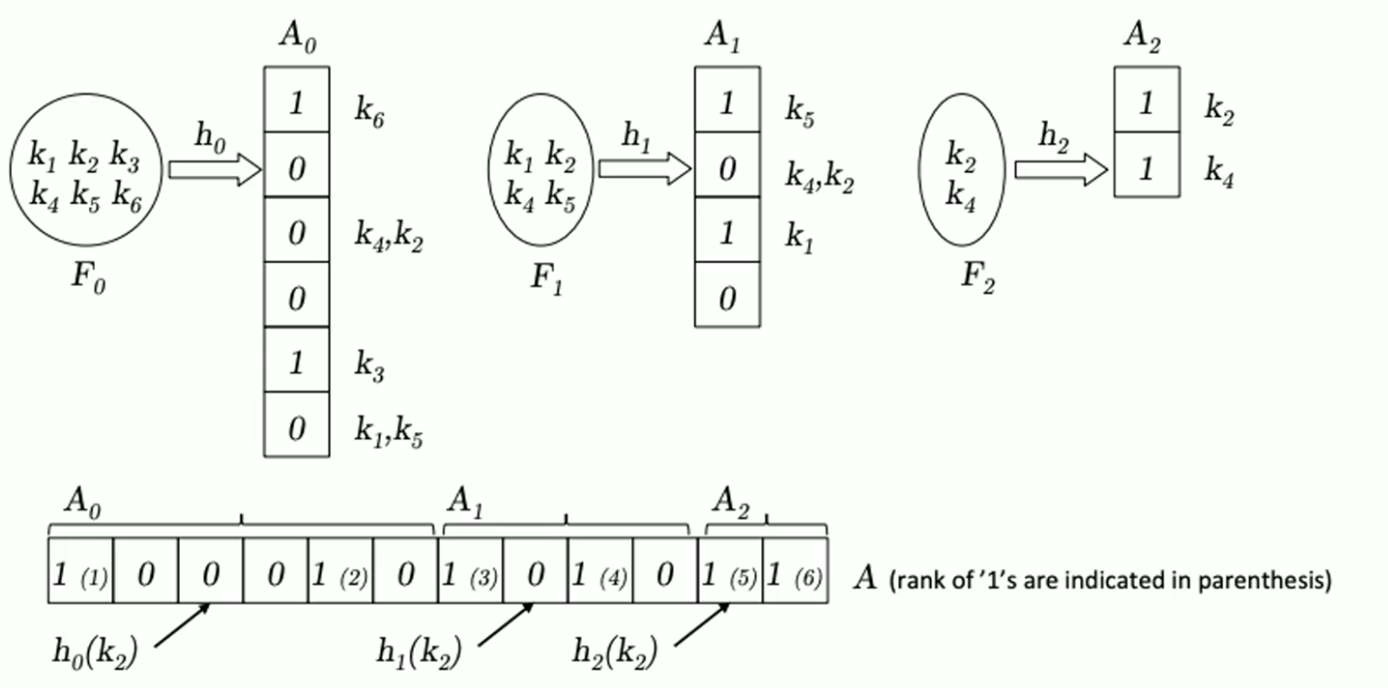
\includegraphics[width=\textwidth]{W2_7.png}
\end{center}
BBHash essentially does many hashes in a row using a classical hash
\begin{itemize}
    \item First hash uses all the $n$ elements with $n$ indices of the resulting table.  
    \item Those entries with collisions or no entries mapped, as well as the elements, are repeated with a second hash.
    \item This pattern continues until there are no collisions left.
    \item The result is the concatenation of all three structures.
    \item To query, you apply the first hash.  If the result is 1, you retrieve the value.  If the result is a 0, you apply the second hash, and go to the next section, etc.
\end{itemize}

\section*{Dynamic Programming}
\begin{itemize}
    \item Go search this up on google, there are many examples of the type of problems, as well as the ways to solve them.
\end{itemize}
\subsection*{Alignment With Dynamic Programming}
\begin{itemize}
    \item Suppose you have two strings \texttt{ATACGTA} and \texttt{ATTACGA}.
    \item The optimal alignment is:
    \begin{verbatim}
        AT-ACGTA
        ATTACG_A
    \end{verbatim}
    \item "edit distance of 2"
    \item How do we find this alignment?
\end{itemize}
\textbf{Steps:}
\begin{enumerate}
    \item To start, let $L$ and $R$ represent the two strings to be aligned.  Let $l$ and $r$ denote the lengths of $L$ and $R$, respectively.  Let $e$ represent the maximum number of errors allowed.
    \item Create a matrix, $M$ with $l + 1 + e$ rows and $r + 1 + e$ columns, representing the indices in each string.
    \item Populate the $0$-th row and column with values of the indices.
    \begin{center}
    \begin{tabular}{|l|l|l|l|l}
        \hline
        \multicolumn{1}{|c|}{0} & \multicolumn{1}{c|}{-1} & -2 & -3 & $\dots$ \\ \hline
        \multicolumn{1}{|c|}{-1} & \multicolumn{1}{c|}{} &  &  & $\dots$ \\ \hline
        -2 &  &  &  & $\dots$ \\ \hline
        -3 &  &  &  & $\dots$ \\ \hline
        $\vdots$ & $\vdots$ & $\vdots$ & $\vdots$ & $\ddots$
    \end{tabular}
    \end{center}
    \item Let $i$ and $j$ be counters for rows and columns, respectively.  Going row by row through the table, fill in each tile at location ($i, j$) following the rules:
    \begin{itemize}
        \item If the character $L_i$ matches $R_j$, then fill $M_{i, j}$ with the value of $M_{i - 1, j - 1} + 1$
        \item If the character does not match, then fill $M_{i, j}$ with MAX$(M_{i - 1, j - 1}$, $M_{i - 1, j}$, $M_{i, j - 1}) - 1$.
    \end{itemize}
    \item Repeat until the bottom right tile is filled.
    \item Backtrack through the graph, starting from the index with the maximum value.
    \begin{itemize}
        \item If the value of $M_{i, j}$ is equal to $M_{i - 1, j - 1} + 1$, then move diagonally up.
        \item Otherwise, move to the cell (either left, up-left, or up) with the highest value.
        \item Assuming you are trying to match $R$ to $L$, ($L$ is the reference)
        \begin{itemize}
            \item Each time you move up left with a $+1$ difference, the letters match
            \item Each time you move left, there was an insertion in $R$.
            \item Each time you move up, there was a deletion in $R$.
            \item Each time you move up left, with a $-1$ difference, there was a substitution in $R$.
        \end{itemize}
    \end{itemize}
    \item Repeat until you reach the beginning of the sequence, the top left corner.
    \item This algorithm is $O(m \cdot n)$.
\end{enumerate}

\section*{Metagenomics: Key Concepts}
\begin{itemize}
    \item A sample contains multiple organisms
    \item Sequencing of the sample obtains reads from each of the present organisms
    \item There is a library of reference genomes available. 
    \item Only a small fraction of the genomes are present in the sample.
    \item A difficulty is that there are repeated regions in the genomes.
    \item A read may match multiple organisms because of the repeats.
\end{itemize}

\subsection*{Metagenomic Formats}
\begin{itemize}
    \item Reference Sequences and reads format is the same as Read Mapping Project
    \item Your goal is to predict the "origin" of each read
\end{itemize}
Left is the read number, right is the genome number it came from.  The goal is to make a guess for every read.
\begin{verbatim}
    >read_0 Genome_Number_85
    >read_1 Genome_Number_67
    >read_2 Genome_Number_91
    >read_3 Genome_Number_85
    >read_4 Genome_Number_85
    >read_5 Genome_Number_73
    >read_6 Genome_Number_63
    >read_7 Genome_Number_91
    >read_8 Genome_Number_99
    >read_9 Genome_Number_63
\end{verbatim}



\end{document}